\chapter{Un ordinateur quantique}\label{ch:un-ordinateur-quantique}

Après avoir présenté la théorie, on va montrer comment cela a été implémenté
dans la réalité.
Notons que ce qui va suivre est principalement pour donner une idée, et non une
description complète et précise de la réalité et des techniques utilisées.

\section{Universalité}\label{sec:universalite}

La notion d'universalité a déjà été évoquée plus haut, et donc tout comme en
informatique classique, on va chercher à trouver un ensemble de portes permettant
de réaliser n'importe quelle opération, dans ce cas avec une précision arbitraire.
Cette limitation de précision est une des raisons de l'apparition d'erreur et de la
nécessité de correction d'erreur.\\
Il existe plusieurs ensembles de portes universels~\cite{universality-proof}, mais on va se concentrer sur
l'ensemble de portes universel de $T = \begin{pmatrix} 1 & 0 \\ 0 & e^{i\pi/4}
\end{pmatrix}$, $H$ et $CX$.\\ \\
Tout d'abord, on va montrer que $T$ et $H$ sont universels permettant de réaliser
n'importe quelle opération sur un seul qubit~\cite{univ-sing,budinger2022alloptical}~.
Premièrement, on va montrer que $T$ et $H$~\cite{hadamard-imp} permettent de réaliser une rotation
d'angle arbitraire autour d'un axe $\hat{n}$.\\
Pour commencer, on a $HTH = R_x(\pi/4)$ et rappelons que $T = R_z(\pi/4)$, ce qui
permet de construire la porte $R_{\hat{n}} = R_z(\pi/4) R_x(\pi/4) = e^{-i\frac{\pi}{8}Z}
e^{-i\frac{\pi}{8}X} = \cos^2 \frac{\pi}{8} I - i \left( \cos \frac{\pi}{8} (X+Z) + \sin
\frac{\pi}{8} Y\right) \sin \frac{\pi}{8}$ (notons que $Y = -i Z X$).\\
C'est une rotation d'axe $\hat{n} = \begin{pmatrix}
\cos \frac{\pi}{8} \\
\sin \frac{\pi}{8} \\
\cos \frac{\pi}{8}
\end{pmatrix}$ sur la sphère de Bloch, avec un angle de rotation donné par
$\cos \frac{\theta}{2} = \cos^2 \frac{\pi}{8} \Rightarrow \theta = 2 \arccos ( \cos^2
\frac{\pi}{8} ) \approx 1.096$ qui n'est pas un multiple rationnel de $2 \pi$.
On peut donc réaliser une rotation d'angle arbitraire autour de l'axe $\hat{n}$ en
appliquant $R_{\hat{n}}$ un nombre arbitraire de fois, car on n'atteindra jamais
un angle multiple de $2 \pi$.
Posons alors $R_{\hat{n}} (\alpha) = R_{\hat{n}}^{n_1}$ avec $n_1 \in \mathbb{N}$.\\
On peut également construire $H R_{\hat{n}} (\alpha) H = R_{\hat{m}} (\alpha)$ avec
$\hat{m} = \begin{pmatrix}
\cos \frac{\pi}{8} \\
-\sin \frac{\pi}{8} \\
\cos \frac{\pi}{8}
\end{pmatrix}$ donc on peut réaliser une rotation d'angle arbitraire autour de
l'axe $\hat{m}$.\\
Finalement, on peut prouver que n'importe quelle porte $U$ peut être écrite comme
\[U = R_{\hat{n}} (\theta_1) R_{\hat{m}} (\theta_2) R_{\hat{n}} (\theta_3) \]
et donc n'importe quelle porte sur un seul qubit peut être réalisée avec une précision
arbitraire avec $T$ et $H$.\\ \\
La porte $CX$~\cite{Rosenblum2018,Noh2018} permet de réaliser une porte $CU$ quelconque, car on peut créer déjà
n'importe quelle porte sur un seul qubit~\cite{univ-double}.\\
Prenons une manière d'écrire une porte générale sur un seul qubit $U(\alpha, \beta,
\gamma, \delta)$ comme suit
\[
    U = e^{i \alpha} \begin{pmatrix}
        e^{-i \frac{\beta + \delta}{2} \cos \frac{\gamma}{2}} & - e^{-i \frac{\beta - \delta}{2} \sin \frac{\gamma}{2}} \\
        e^{i \frac{\beta - \delta}{2} \sin \frac{\gamma}{2}} & e^{i \frac{\beta + \delta}{2} \cos \frac{\gamma}{2}}
    \end{pmatrix}
\]
qui permet de réécrire $U$ comme $U = e^{i \alpha} A X B X C$ avec
$X$ la porte de Pauli $X$ et $A, B, C$ des portes sur un seul qubit, dont on peut
passer le détail de leur construction algébrique, mais qui peuvent être précisément
déterminées et donc implémentées.\\
En posant aussi $D = \begin{pmatrix}
1 & 0 \\
0 & e^{i \alpha}
\end{pmatrix}$, on peut construire la porte $CU$ comme suit
\begin{figure}[H]
    \centering
    \[\shorthandoff{!}
    \scalebox{1.0}{
        \Qcircuit @C=1.0em @R=0.2em @!R { \\
         & \ctrl{1} & \qw\\
         & \gate{U} & \qw\\
        \\ }}
    \]
    =
    \[\shorthandoff{!}
    \scalebox{1.0}{
        \Qcircuit @C=1.0em @R=0.2em @!R { \\
         & \qw & \ctrl{1} & \qw & \ctrl{1} & \gate{D} & \qw\\
         & \gate{C} & \targ & \gate{B} & \targ & \gate{A} & \qw\\
        \\ }}
    \]
    \caption{Circuit d'une porte $CU$}
    \label{fig:control-u}
\end{figure}
où l'on voit la porte $D$ sur le qubit de contrôle, car la phase globale de la porte
$U$ va impacter le qubit de contrôle, et doit donc être prise en compte par l'ajout
de la porte $D$.\\ \\
On peut ensuite se convaincre qu'à partir de n'importe quelle porte $U$ sur un seul
qubit, et porte contrôlée $CU$, on peut construire n'importe quelle porte sur $n$
qubits.
La démonstration est néanmoins trop complexe pour être présentée ici.

\section{Hardware}\label{sec:hardware-quantique}

La création d'ordinateurs quantiques est un défi technologique majeur, car il faut
pouvoir manipuler des qubits, qui sont des systèmes quantiques, avec une précision
extrême, et ce, à grande échelle.\\
Plusieurs facteurs compliquent la tâche, comme la décohérence qui fait que les
qubits perdent leur état quantique et donc leurs avantages au bout d'un
certain temps (de l'ordre de la microseconde pour les qubits supraconducteurs, sinon
des dizaines de nanosecondes en général), ou encore le fait que les qubits doivent
être isolés de leur environnement pour éviter les erreurs de mesure, ce qui
nécessite des températures très basses (moins d'un Kelvin).\\ \\
Une des implémentations les plus avancées~\cite{wiki:ibm-quantum} est celle des qubits supraconducteurs~\cite{wiki:superconducting-qc},
ou qubit de charge~\cite{wiki:charge-qbit}, qui sont des qubits dont l'état est codé dans la charge d'un
condensateur supraconducteur~\cite{wiki:transmon,wiki:trapped-ion}.\\
Un supraconducteur est un matériau qui, en dessous d'une certaine température
critique, n'a plus de résistance électrique.
La méthode de fabrication des qubits de charge est similaire à celle des autres
circuits de microélectronique, en gravant du silicium ou du saphir avec des
techniques de lithographie par électrons.
Ils utilisent des métaux tel que le niobium ou le tantale.\\
Le dernier point de construction est les jonctions Josephson~\cite{wiki:josephson-effect}, qui sont des
jonctions entre deux supraconducteurs séparés par une barrière isolante, qui
est dans ce cas un oxyde d'aluminium.
La méthode de création de ces jonctions est grossièrement la création d'un masque
sur le supraconducteur, puis en évaporant le métal à différents angles par le masque.\\ \\
Le qubit se compose donc d'un condensateur supraconducteur, d'une jonction Josephson
et d'une tension qui permet de contrôler la charge du condensateur.
\import{images/notions-bases/hardware/}{charge-qubit.tex}
La région en traitillé représente une ``île'' de supraconducteur, qui est
une région isolée de par le fait qu'une énergie est nécessaire à une charge
pour y entrer.
Néanmoins, les particules peuvent passer par effet tunnel, qui est dû à la
mécanique quantique, et à la nature ondulatoire des particules.
De manière classique, une particule ne pourrait pas passer la barrière d'énergie,
mais l'équation d'onde de la particule permet de calculer une probabilité de
passage, qui est non nulle.
Pour les électrons, on arrive à mesurer le passage d'une barrière de quelques
nanomètres d'épaisseur, ce qui donne une idée de la précision nécessaire pour
la fabrication des qubits.\\
La jonction Josephson est cette barrière qui va créer un effet tunnel entre
les deux supraconducteurs.
Les objets quantiques dont on mesure le passage sont des paires de Cooper,
qui sont des paires d'électrons liés par une interaction attractive.
Celles-ci se forment dans les supraconducteurs, et peuvent être en quelque sorte
décrites par une analogie classique.
Les électrons sont des particules chargées négativement, et donc se repoussent.
Or étant négatif, ils attirent les ions positifs du réseau cristallin du
supraconducteur, ce qui crée une déformation du réseau.
Cela va créer une densité de charge positive, qui va pouvoir attirer un autre
électron, et si l'attraction est plus forte que la répulsion, les deux électrons
vont être liés et former une paire de Cooper~\cite{wiki:cooper-pair}.
Dès lors, le qubit qui représente l'état $\ket{0}$ serait l'absence de paire de Cooper dans l'île
et l'état $\ket{1}$ serait la présence de celles-ci. \\ \\
Pour manipuler ces qubits, que ce soit appliquer une porte ou le mesurer, on va utiliser
des micro-ondes, qui sont des ondes électromagnétiques.
En envoyant des micro-ondes à une fréquence précise et selon un pattern précis~\cite{gate-impl},
on va pouvoir modifier l'évolution du système, ce qui correspond à ce
que l'on a appelé une porte quantique.\\
Pour la mesure, on va regarder les fréquences de résonance du système, soit les
fréquences que le qubit réfléchit qui sont caractéristiques de son état.\\
On peut également créer une porte contrôlée en envoyant des micro-ondes sur un
qubit avec une fréquence de résonance avec un deuxième qubit, ce qui va
créer une rotation de l'état du deuxième qubit autour de l'axe $x$ sur la sphère
de Bloch.
La direction de la rotation va dépendre de l'état du premier qubit, et donc on
a une porte contrôlée.
Notons que pour cela, il faut que les deux qubits soient reliés par ce que l'on
appelle un bus, qui est grossièrement une cavité faisant résonner les micro-ondes
à l'intérieur, et qui relie les deux qubits.\\ \\
\begin{figure}[H]
    \centering
    \subfloat[Qubits]{
        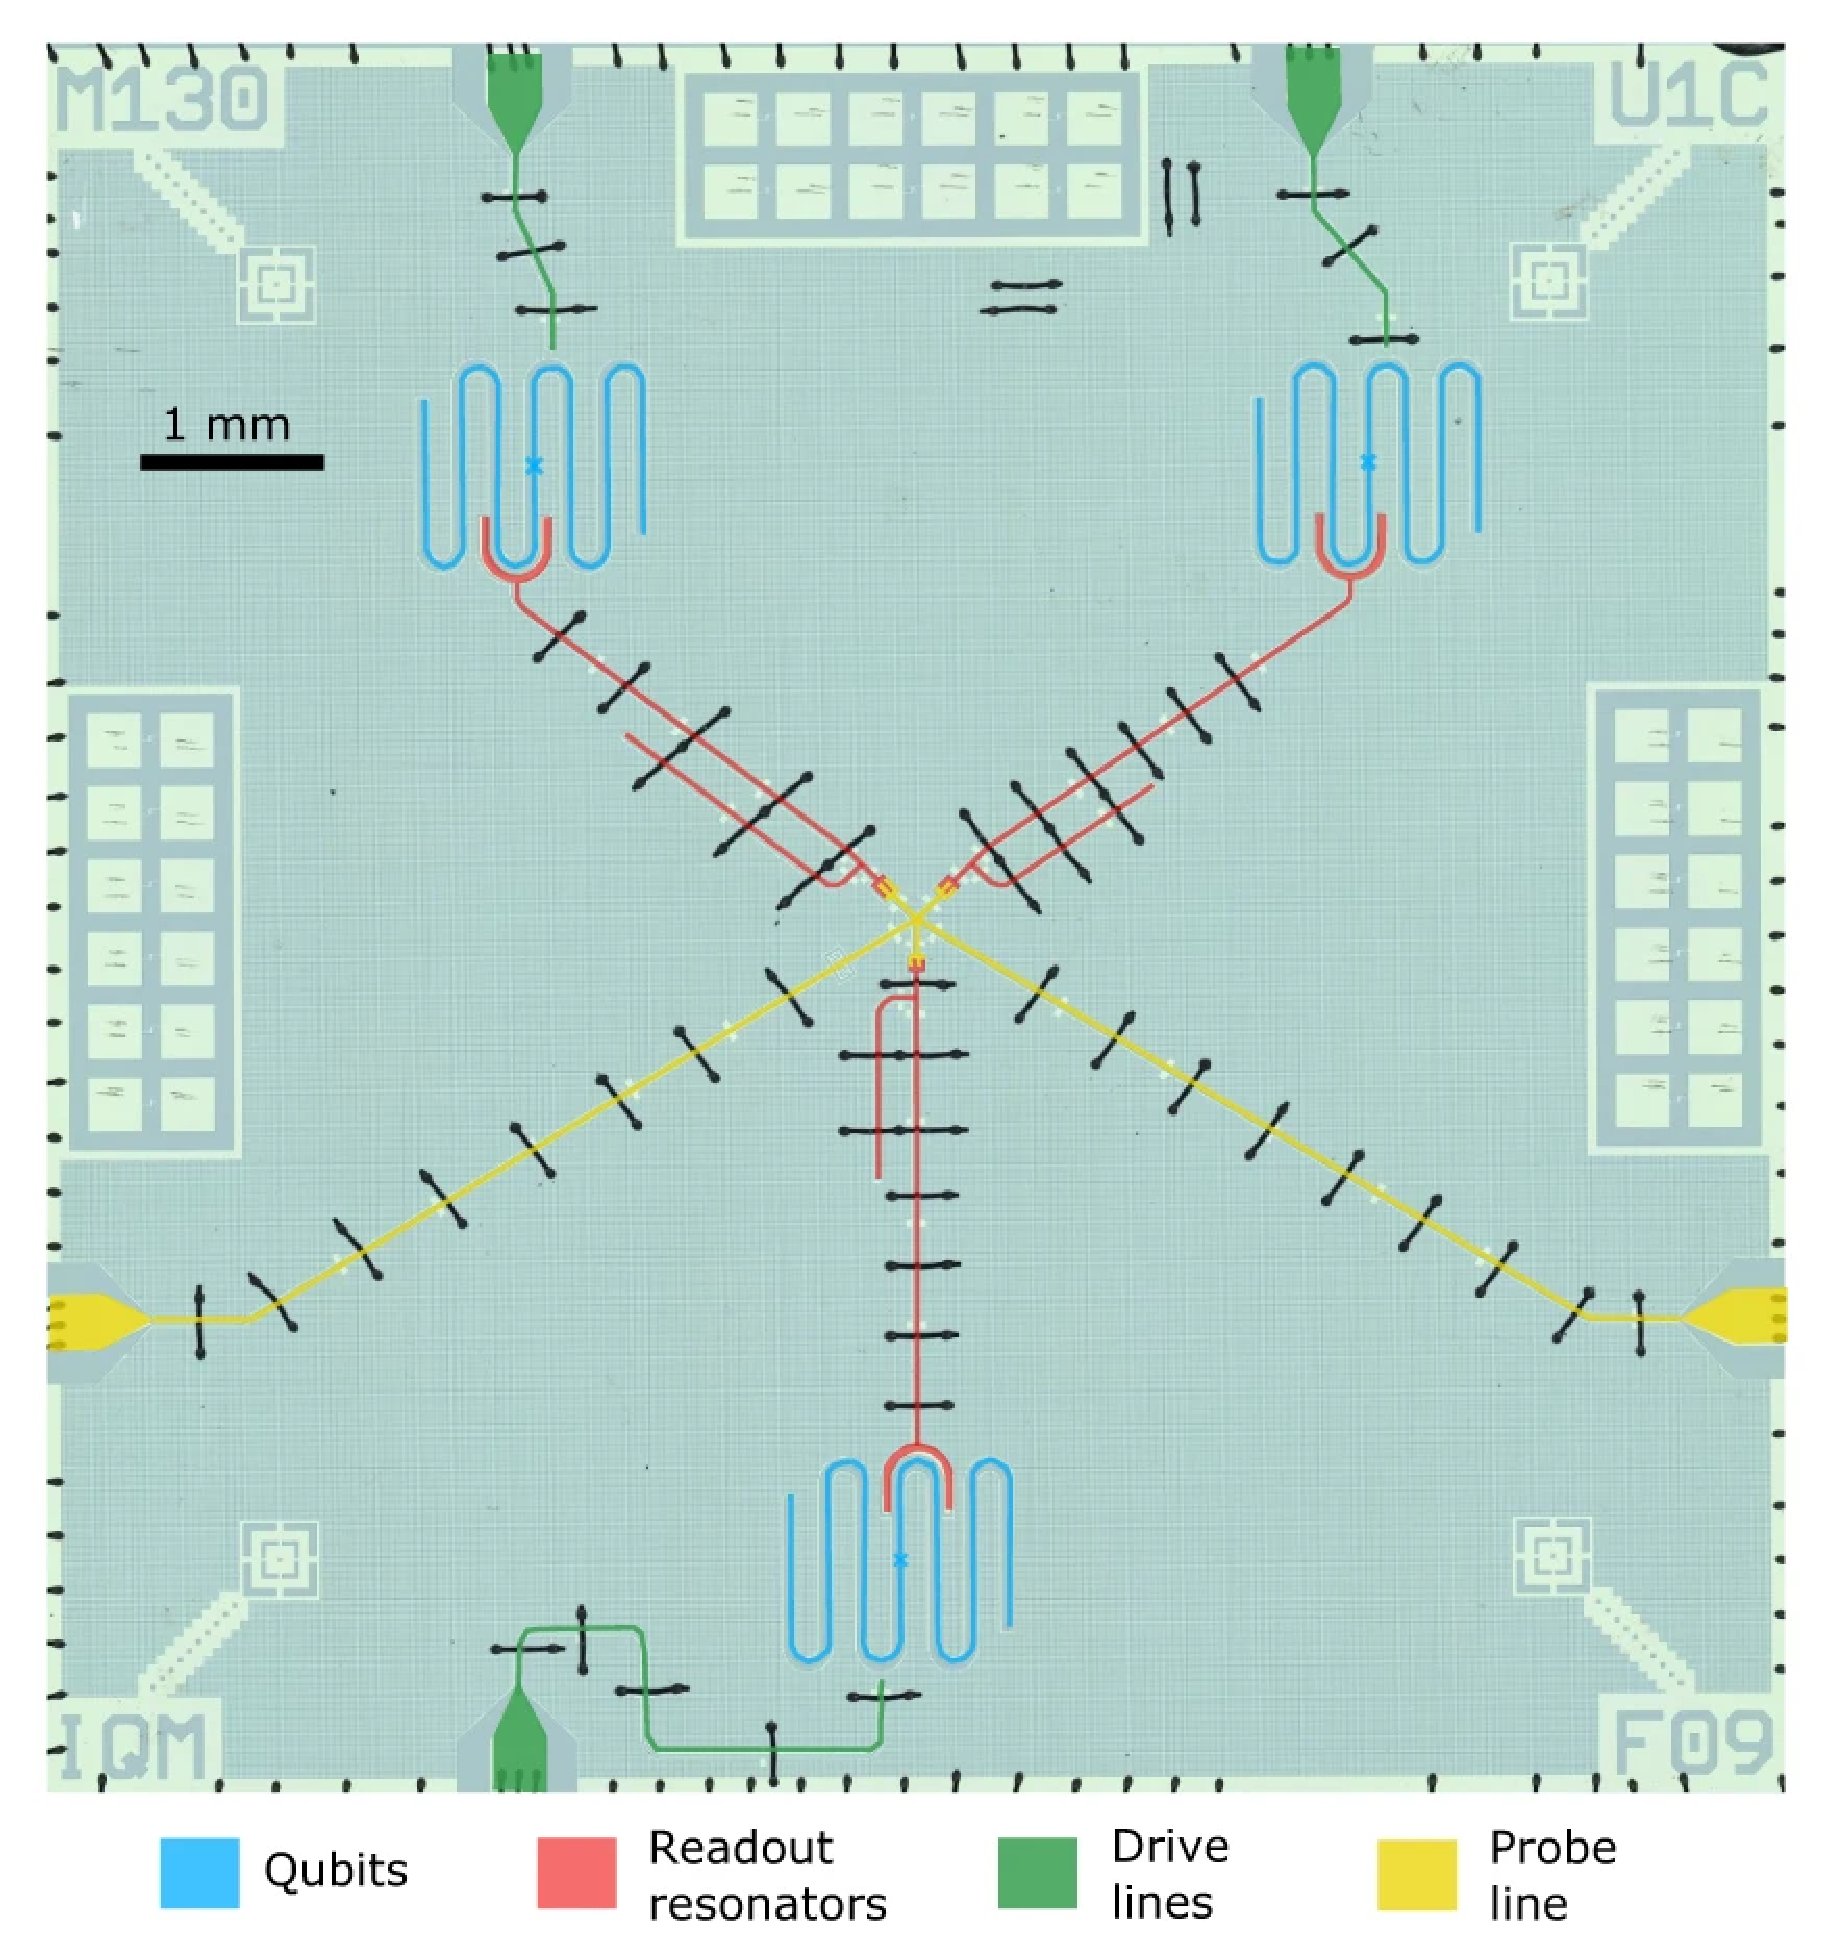
\includegraphics[width=0.4\textwidth]{images/notions-bases/hardware/qubit-micro.eps}
    }
    \subfloat[Électronique externe]{
        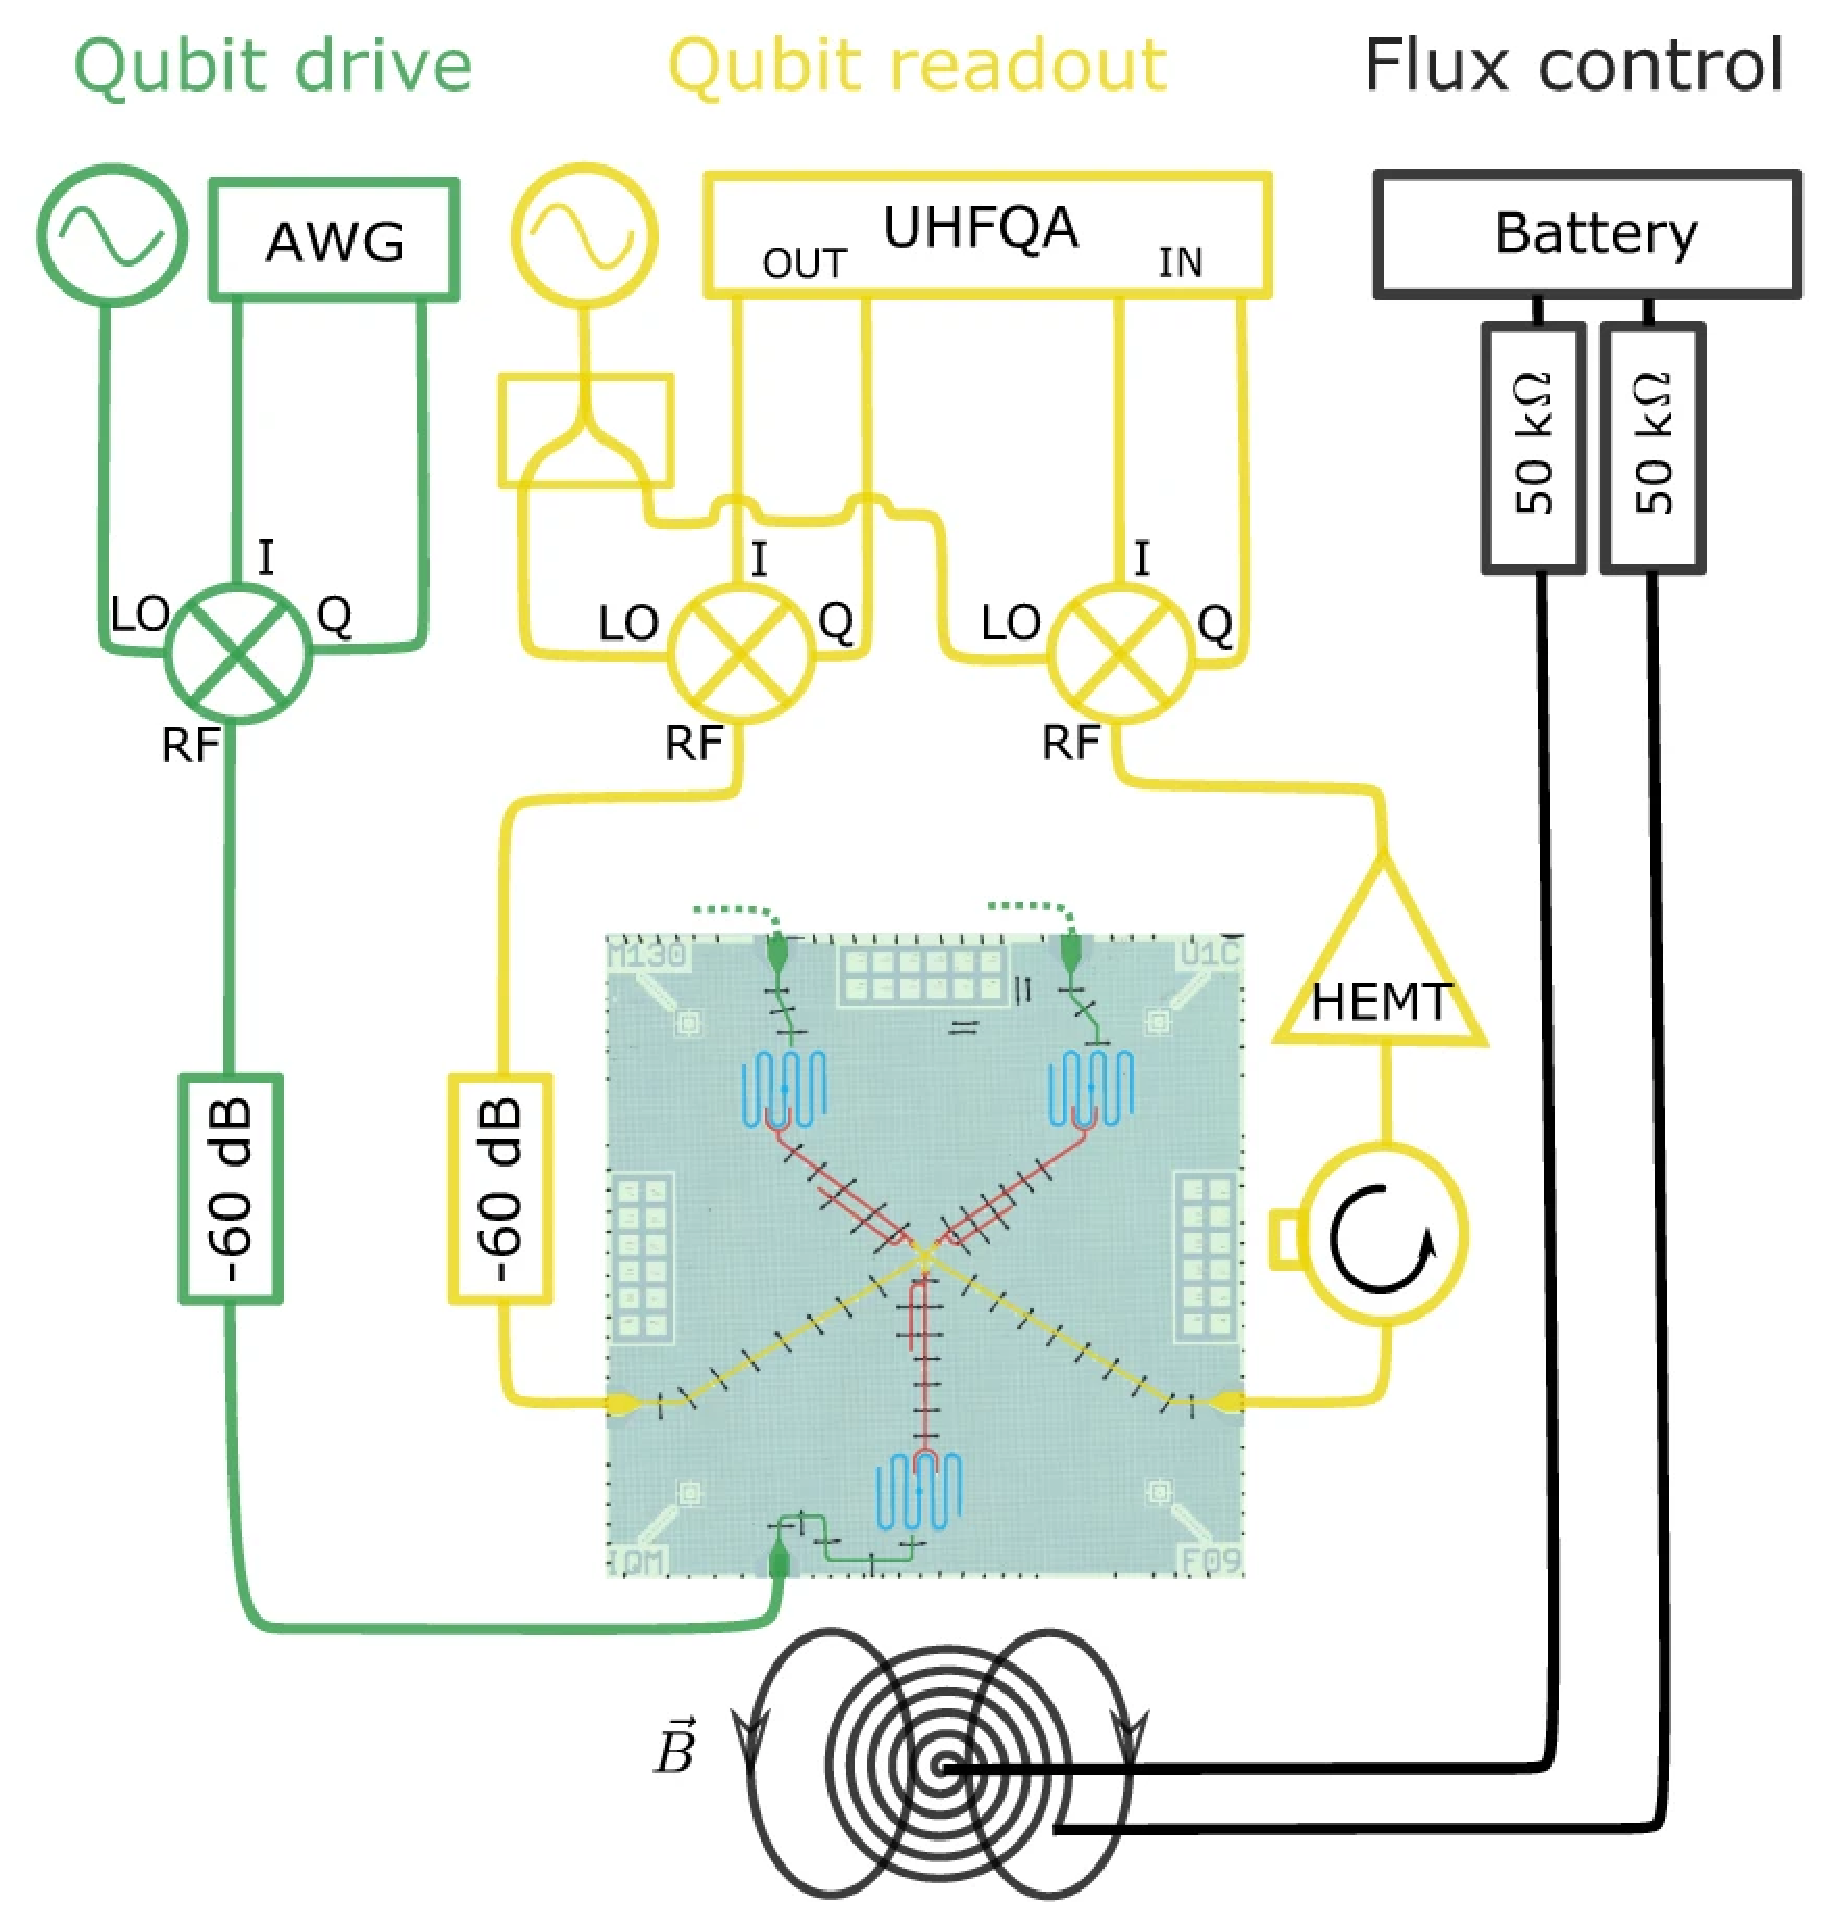
\includegraphics[width=0.4\textwidth]{images/notions-bases/hardware/qubit-exp.eps}
    }
    \caption{Image au microscope colorisée de qubits ainsi que le dispositif électronique pour son utilisation~\cite{Hyypp2022}}
    \label{fig:qubit-microscope}
\end{figure}
Cette revue de la technologie actuelle est très simplifiée, et ne donne qu'un
aperçu de la complexité de la fabrication d'un ordinateur quantique, tant de
par la recherche fondamentale nécessaire pour comprendre les phénomènes
quantiques, que de par la technologie nécessaire pour manipuler ces phénomènes
à grande échelle.
Notons que de plus, la puce à proprement parler ne mesure guère plus de quelques
centimètres carrés, mais que pour son bon fonctionnement, il faut qu'elle soit
proche du zéro absolu pour préserver les propriétés supraconductrices des
matériaux, et il faut l'isoler complètement de l'environnement afin d'éviter
la décohérence du système, donc il faut créer un vide presque parfait et l'isoler
de la lumière et des ondes électromagnétiques entre autres.
\import{images/notions-bases/hardware/}{arch-qc.tex}
Sur la figure~\ref{fig:archi}, on peut voir une architecture simplifiée d'un
ordinateur quantique, avec principalement la zone protégée avec l'ordinateur
quantique à proprement parler, sur laquelle sont figurées différentes parois de
protection en gris, ainsi que la tour de refroidissement en jaune.
Celle-ci fait en pratique plus d'un mètre de haut, et tout en bas de celle-ci se trouve
la puce.
En vert, les câbles de contrôle, qui représente les micro-ondes envoyées sur
les qubits pour les manipuler, et en bleu et rouge ceux du système de refroidissement.
On y voit également la nécessité de systèmes externes à l'ordinateur quantique afin
de l'utiliser, comme un ordinateur classique pour contrôler les micro-ondes,
ainsi que des systèmes de refroidissement et de pompage du vide, d'autres
de contrôles et de mesures, etc.
L'utilisation de ces ordinateurs quantiques se fait donc à distance pour le grand
public, si on peut parler de grand public, et cette manière de faire est celle
privilégiée par les entreprises qui proposent des ordinateurs quantiques même dans
le développement de ceux-ci, car en avoir un chez soi n'est vraisemblablement pas
utile, comme on le verra dans les utilisations possibles de ces ordinateurs.\\ \\
Un ordinateur quantique est un système très complexe, nécessitant une isolation
parfaite de l'environnement pour bien fonctionner, et donc il est très difficile
de créer un ordinateur quantique avec un grand nombre de qubits.
Cela explique aussi qu'actuellement, les ordinateurs quantiques ne sont pas encore
parfaits, mais on peut déjà faire des expériences avec quelques qubits, et
espérer que ceux-ci seront de plus en plus performants dans le futur.
Dans un ordinateur classique, la logique est réalisée par des transistors dans lesquels
passent un courant électrique, alors que dans un ordinateur quantique, on a un
système quantique sur lequel on applique des opérations modifiant son état.
De part cette différence, le qubit contient son information dans son état, à la
différence d'un bit classique qui doit être enregistré dans un système externe
pour être conservé.